\section{PTracking Algorithm}

\begin{frame}
	\frametitle{Distributed Particle Filtering for Multi-Agent Multi-Object Tracking}
	
	\Large
	
	\begin{block}{Idea}
		Achieving both a \textbf{high} precision and a \textbf{high} robustness, as a
		global method does, while keeping a \textbf{low} computational load in order to
		obtain \textbf{real-time} performance, as recursive methods do
	\end{block}
\end{frame}

\begin{frame}
	\frametitle{PTracking algorithm}
	
	\begin{columns}[T]
		\column{.5\textwidth}
		
		\vspace{0.8cm}
		
		\begin{itemize}
			\item \textbf{Input:} a set of positions of the objects provided by a multi object
				  detection system
			
			\vspace{1.6cm}
			
			\item \textbf{Output:} a set of estimated trajectories of the moving objects over
				  time
		\end{itemize}
		
		\column{.5\textwidth}
		\centering
		
		\begin{tikzpicture}
			\node at (0,0) [draw=black,ultra thick,inner sep=0pt]
			{
				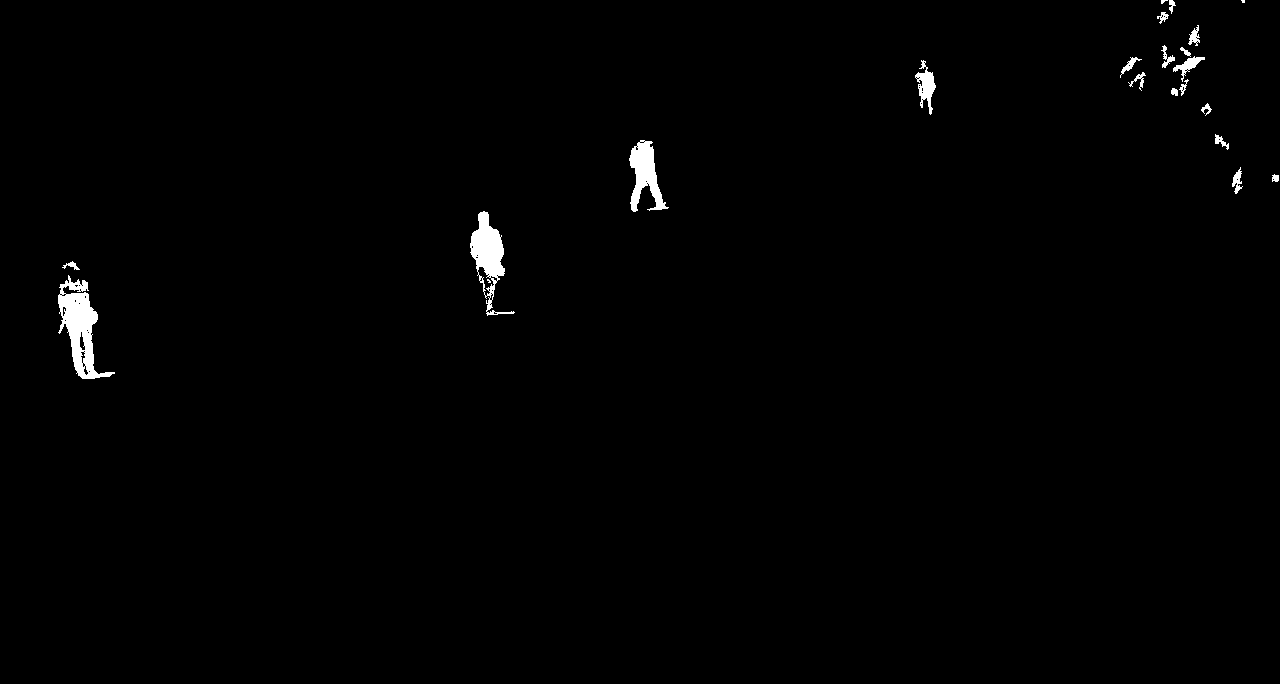
\includegraphics[width=6cm]{Figures/Detection.png}
				
			};
			\node at (0,-3.35) [draw=black,ultra thick,inner sep=0pt]
			{
				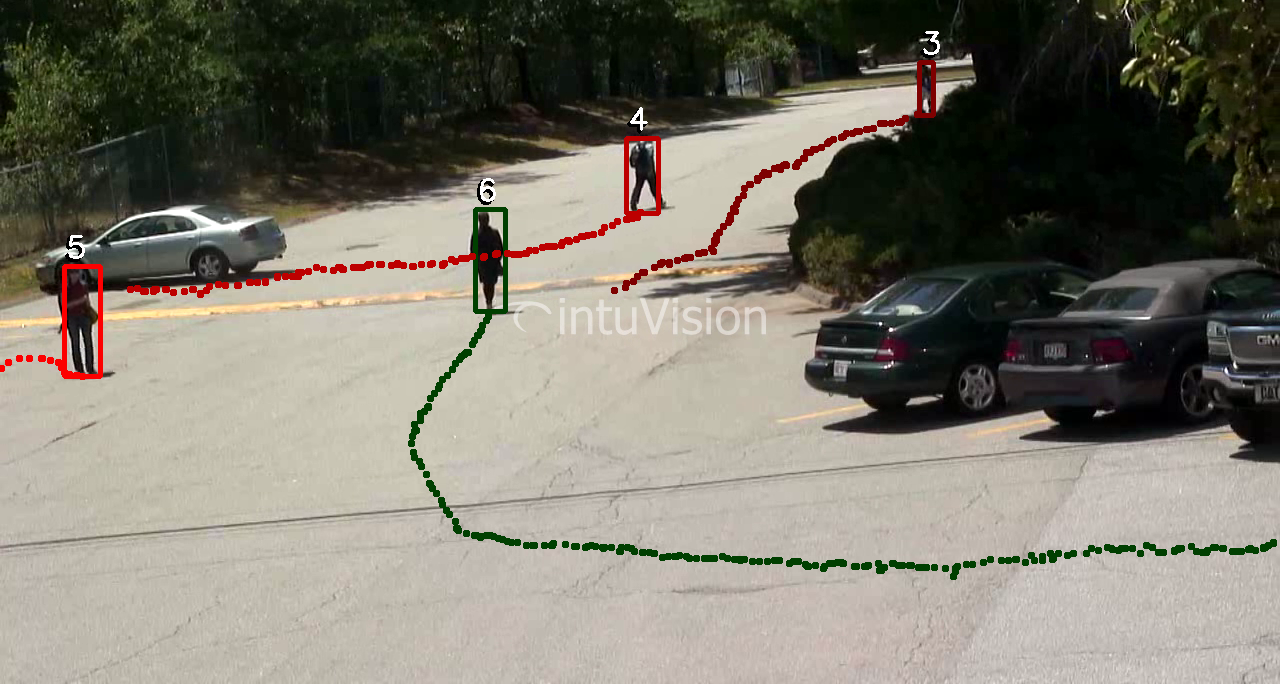
\includegraphics[width=6cm]{Figures/Tracking.png}
				
			};
		\end{tikzpicture}
	\end{columns}
\end{frame}

\begin{frame}
	\frametitle{PTracking algorithm}
	\framesubtitle{Informal formulation}
	
	\only<1->
	{
		\large
		Each agent runs a two-tiered distributed algorithm
	}
	
	\begin{columns}
		\column{0.4\textwidth}
		\centering
		
		\only<1->
		{
			\vspace{0.7cm}
		}
		
		\only<1->
		{
			\begin{tikzpicture}
				\node at (0,0) [draw=black,ultra thick,inner sep=0pt]  {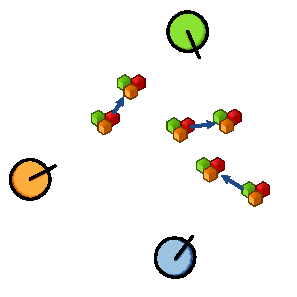
\includegraphics[scale=0.75]{Figures/Mamot}};
			\end{tikzpicture}
		}
		
		\column{0.2\textwidth}
		\centering
		
		\only<2->
		{
			\begin{tikzpicture}
				\node at (0,0) [draw=white,ultra thick,inner sep=0pt]  {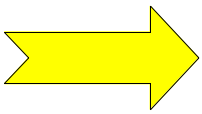
\includegraphics[scale=0.3]{Figures/ArrowRight.png}};
			\end{tikzpicture}
		}
		
		\column{0.4\textwidth}
		\centering
		
		\only<2>
		{
			\begin{tikzpicture}
				\node at (0,0) [draw=black,ultra thick,inner sep=0pt]  {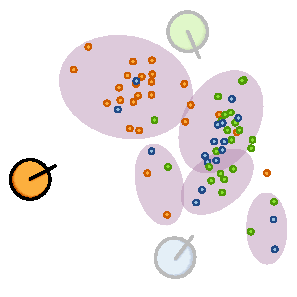
\includegraphics[scale=0.75]{Figures/Mamot2}};
			\end{tikzpicture}
		}
		
		\only<2>
		{
			\vspace{-0.7cm}
		}
		
		\only<3>
		{
			\begin{tikzpicture}
				\node at (0,0) [draw=black,ultra thick,inner sep=0pt]  {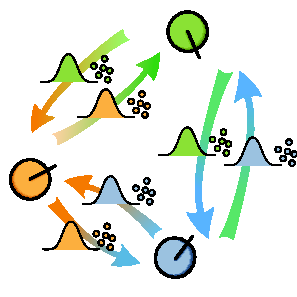
\includegraphics[scale=0.75]{Figures/Mamot3}};
			\end{tikzpicture}
		}
		
		\only<3>
		{
			\vspace{-0.7cm}
		}
		
		\only<4>
		{
			\begin{tikzpicture}
				\node at (0,0) [draw=black,ultra thick,inner sep=0pt]  {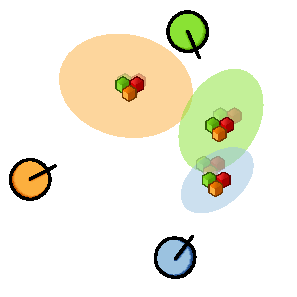
\includegraphics[scale=0.75]{Figures/Mamot4}};
			\end{tikzpicture}
		}
		
		\only<4>
		{
			\vspace{-0.7cm}
		}
	\end{columns}
\end{frame}

\begin{frame}
	\frametitle{PTracking algorithm}
	\framesubtitle{Mathematical formulation}
	
	\vspace{0.4cm}
	
	\textbf{Global recursive update}
	
	\vspace{-0.4cm}
	
	\begin{eqnarray*}
	p(x_t|z_{1:t-1}^\mathcal{A}) &=& \int p(x_t|x_{t-1}) p(x_{t-1}|z_{1:t-1}^\mathcal{A})dx_{t-1}, \\
	p(x_t|z_{1:t}^\mathcal{A}) &=& \frac{p(z_t^\mathcal{A}|x_t) p(x_t|z_{1:t-1}^\mathcal{A})}{\int p(z_t^\mathcal{A}|x_t)p(x_t|z_{1:t-1}^\mathcal{A})dx_t}.
	\end{eqnarray*}
	
	\textbf{GMM parameters}
	
	\vspace{-0.1cm}
	
	\begin{equation*}
		\mu_t^c = \frac{\sum_{i=1}^N x_t^{(i)}\lambda_t(c|x_t^{(i)})}{\sum_{i=1}^N \lambda_t(c|x_t^{(i)})},\;\;\;\;\;\;\;
		\sigma_t^c = \frac{\sum_{i=1}^N (x_t^{(i)} - \mu_t^c)^2\lambda_t(c|x_t^{(i)}) }{\sum_{i=1}^N \lambda_t(c|x_t^{(i)}) }.
	\end{equation*}
	
	\emph{where}
	
	\vspace{-0.5cm}
	
	\begin{equation*}
		\lambda_t(c|x_t^{(i)}) = \frac{\mathcal{N}(x_t^{(i)},\mu_t^c,\sigma_t^c)\lambda_t^c} {\sum_{m=1}^{\mathcal{C}}\mathcal{N}(x_t^{(i)},\mu_t^m,\sigma_t^m)\lambda_t^m},\;\;\;\;\;\;\;
		\lambda_t^c = \frac{1}{N} \sum_{i=1}^N \lambda_t(c|x_t^{(i)}),
	\end{equation*}
\end{frame}

\begin{frame}
	\frametitle{PTracking algorithm}
	\framesubtitle{Pseudo-code}
	
	\vspace{0.35cm}
	
	\begin{algorithm}[H]
		\tiny
		\caption{PTracking}
		\KwIn{perceptions $ z_{s,t} $, local track numbers $ oi_{s,t-1} $, global track numbers $ OI_{s,t-1} $}
		\BlankLine
		\KwData{set of local particles $ \tilde{\xi}_{s,t} $, set of global particles $ \tilde{\xi}_{\mathcal{S'},t} $, local GMM set $ \mathcal{L} $, global GMM set $ \mathcal{G} $}
		\BlankLine
		\KwOut{global estimations $ x_{s,t} = (\boldsymbol{OI}_{s,t},\boldsymbol\Lambda_{s,t},\boldsymbol{M}_{s,t},\boldsymbol\Sigma_{s,t}) $}
		\BlankLine
		\Begin
		{
			$ \tilde{\xi}_{s,t} \sim \pi_t (x_{s,t} | x_{s,t-1},z_{s,t}) $
			\BlankLine
			Re-sample by using the SIR principle\\
			\BlankLine
			$ \mathcal{L} = KClusterize(\tilde{\xi}_{s,t}) $
			\BlankLine
			$ (\boldsymbol{oi}_{s,t},\boldsymbol\lambda_{s,t},\boldsymbol\mu_{s,t},\boldsymbol\sigma_{s,t}) = DataAssociation(\mathcal{L}, oi_{s,t-1}) $
			\BlankLine
			Communicate the belief $ (\boldsymbol{oi}_{s,t},\boldsymbol\lambda_{s,t},\boldsymbol\mu_{s,t},\boldsymbol\sigma_{s,t}) $ to the other cameras
		}
		\BlankLine
		\Begin
		{
			Collect $ \mathcal{L}_{S'} $ from a subset $ \mathcal{S'} \subseteq \mathcal{S} $ of the cameras within a period $ \Delta t $
			\BlankLine
			$ \tilde{\xi}_{\mathcal{S'},t} \sim \tilde\pi = \sum_{s \in \mathcal{S'}} \boldsymbol\lambda_{s,t} \, \mathcal{N} (\boldsymbol\mu_{s,t},\boldsymbol\sigma_{s,t}) $
			\BlankLine
			Re-sample by using the SIR principle\\
			\BlankLine
			$ \mathcal{G} = KClusterize(\tilde\xi_{{\mathcal{S'},t}}) $
			\BlankLine
			$ (\boldsymbol{OI}_{s,t},\boldsymbol\Lambda_{s,t},\boldsymbol{M}_{s,t},\boldsymbol\Sigma_{s,t}) = DataAssociation(\mathcal{G},OI_{s,t-1}) $
		}
	\end{algorithm}
\end{frame}

\begin{frame}
	\frametitle{PTracking algorithm}
	\framesubtitle{Group tracking}
	
	
	\begin{figure}
		\begin{tikzpicture}[map/.style={draw=black,ultra thick,inner sep=0pt}]
			\node at (0,0) [map] {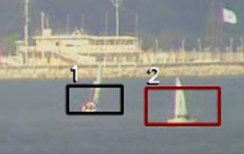
\includegraphics[width=0.32\linewidth]{Figures/GroupTracking-a}};
			\node at (4,0) [map] {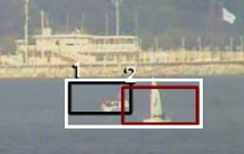
\includegraphics[width=0.32\linewidth]{Figures/GroupTracking-b}};
			\node at (8,0) [map] {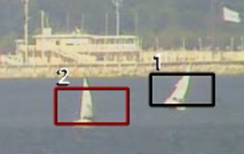
\includegraphics[width=0.32\linewidth]{Figures/GroupTracking-c}};
		\end{tikzpicture}
		\caption{Group tracking. Two sailing boats are going to cross each other. Occlusions are handled considering
				 the collapsing tracks to form a group, instead of tracking them separately.}
	\end{figure}
\end{frame}

\begin{frame}
	\frametitle{Evaluating a Tracking Algorithm}
	
	\Large
	
	\vspace{0.3cm}
	
	The CLEAR MOT (Kasturi \emph{et al.}) metrics \emph{MOTA} and \emph{MOTP} are the de-facto
	standard for evaluating a tracking method:
	
	\vspace{0.2cm}
	
	\large
	
	\begin{equation*}
		MOTA = 1 - \frac{\sum_{t=1}^{N_{frames}} (c_m(m_t) + c_f(fp_t) + cs(ID\mbox{-}SWITCHES_t))}{\sum_{t=1}^{N_{frames}} N_G^{(t)}}
	\end{equation*}
	
	\vspace{0.4cm}
	
	\begin{equation*}
		MOTP = \frac{\sum_{i=1}^{N_{mapped}} \sum_{t=1}^{N_{frames}^{(t)}} \Big [ \frac{| G_i^{(t)} \cap D_i^{(t)} |}{| G_i^{(t)} \cup D_i^{(t)} |} \Big ] }{\sum_{t=1}^{N_{frames}} N_{mapped}^{(t)}}
	\end{equation*}
\end{frame}

\begin{frame}
	\frametitle{Application Field}
	
	\vspace{0.01cm}
	
	\begin{itemize}
		\item Single-Agent, Multi-Object
	\end{itemize}
	
	\vspace{-0.45cm}
	
	\begin{columns}[t]
		\only<1->
		{
			\column{0.75\textwidth}
			
			\begin{block}{Boat visual tracking}
				automatic surveillance system in the maritime domain
			\end{block}
			
			\column{0.2\textwidth}
		}
	\end{columns}
	
	\centering
	\vspace{0.3cm}
	
	\begin{center}
		\begin{tikzpicture}
			\node at (0,0) [draw=black,ultra thick,inner sep=0pt]  {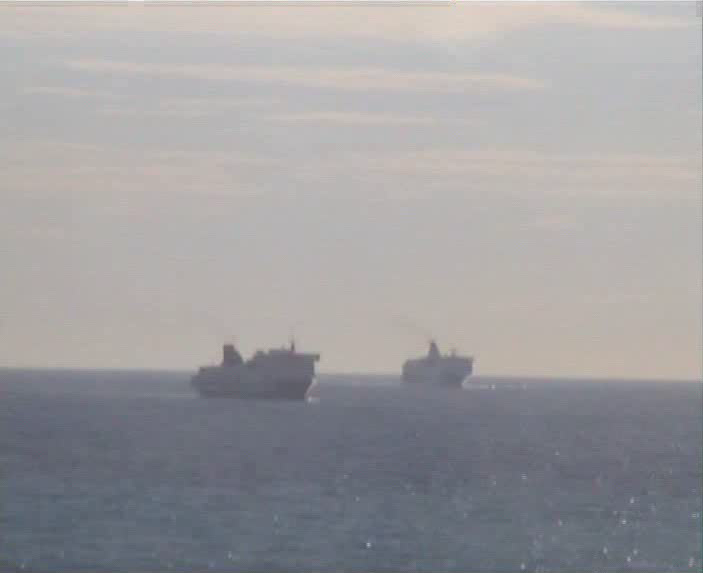
\includegraphics[height=3.1cm]{Figures/Boat-1}};
			\node at (4,0) [draw=black,ultra thick,inner sep=0pt]  {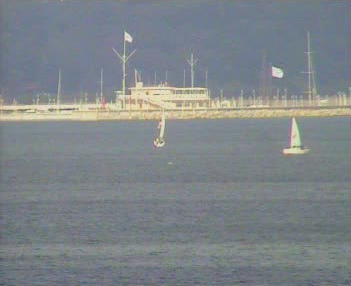
\includegraphics[height=3.1cm]{Figures/Boat-2}};
			\node at (8,0) [draw=black,ultra thick,inner sep=0pt]  {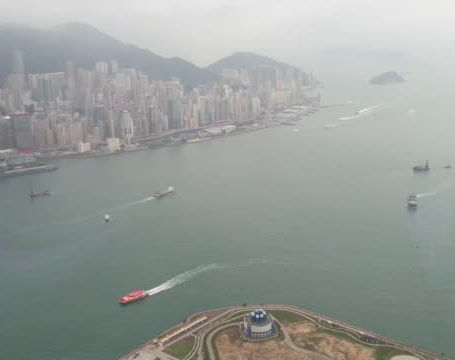
\includegraphics[height=3.1cm]{Figures/Boat-3}};
		\end{tikzpicture}
	\end{center}
\end{frame}

\begin{frame}
	\frametitle{Qualitative Evaluation on the Maritime Domain}
	\framesubtitle{Blue water}
	
	\begin{center}
		\href{run:../Scripts/boat-1.sh}
		{
			\begin{tikzpicture}
				\node at (0,0) [draw=black,ultra thick,inner sep=0pt]
				{
					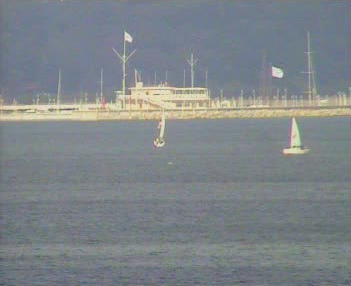
\includegraphics[width=0.65\linewidth]{Figures/Boat-2.png}
				};
			\end{tikzpicture}
		}
	\end{center}
\end{frame}

\begin{frame}
	\frametitle{Qualitative Evaluation on the Maritime Domain}
	\framesubtitle{Honk-Kong port}
	
	\begin{center}
		\href{run:../Scripts/boat-2.sh}
		{
			\begin{tikzpicture}
				\node at (0,0) [draw=black,ultra thick,inner sep=0pt]
				{
					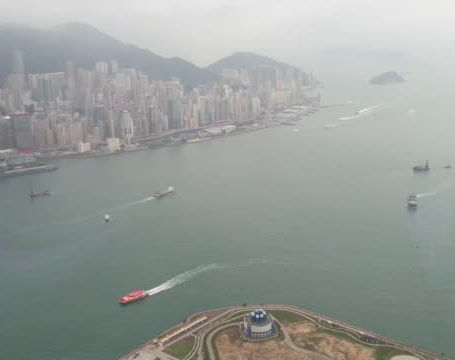
\includegraphics[width=0.65\linewidth]{Figures/Boat-3.png}
				};
			\end{tikzpicture}
		}
	\end{center}
\end{frame}

\begin{frame}
	\frametitle{Quantitative Evaluation on the Maritime Domain}
	
	\begin{table}[!t]
		\renewcommand{\arraystretch}{1.3}
		\caption{Tracking performance on the maritime domain. MOTA (larger the better)
				 considers the number of missed detections, the number of false positives
				 and the switches of identities. MOTP (larger the better) considers the
				 precision of the detections.}
		\centering
		\vspace{0.2cm}
		
		\begin{tabular}{ccc}
			\hline
			\hline
			\textbf{Video} & \textbf{MOTA} & \textbf{MOTP} \\
			\hline
			occlusions-1.avi & 0.815 & 0.613 \\
			\hline
			occlusions-2.avi & 0.910 & 0.554 \\
			\hline
			high-view.avi & 0.910 & 0.604 \\
			\hline
		\hline
		\end{tabular}
	\end{table}
\end{frame}

\begin{frame}
	\frametitle{Qualitative Evaluation on the People Domain}
	\framesubtitle{Park Monitoring}
	
	\begin{center}
		\href{run:../Scripts/people.sh}
		{
			\begin{tikzpicture}
				\node at (0,0) [draw=black,ultra thick,inner sep=0pt]
				{
					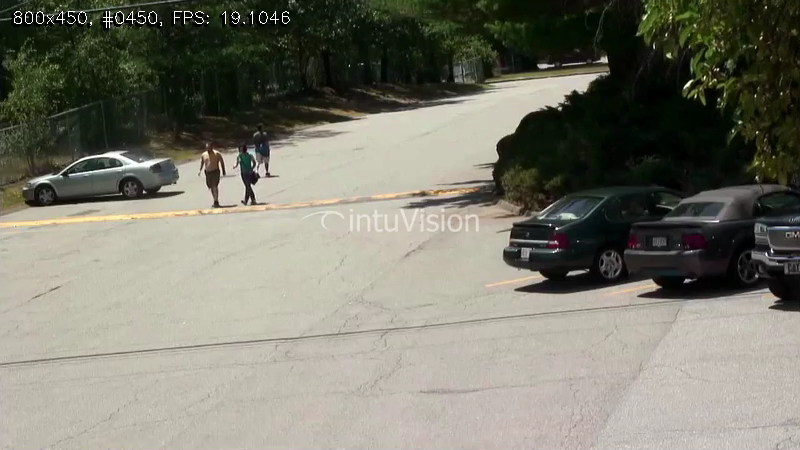
\includegraphics[width=0.65\linewidth]{Figures/People.png}
				};
			\end{tikzpicture}
		}
	\end{center}
\end{frame}

\begin{frame}
	\frametitle{Application Field}
	
	\vspace{0.24cm}
	
	\begin{itemize}
		\item Multi-Agent, Single-Object
	\end{itemize}
	
	\vspace{-0.45cm}
	
	\begin{columns}[t]
		\only<1->
		{
			\column{0.75\textwidth}
			
			\begin{block}{Soccer robots}
				used to solve the localization field symmetry problem
			\end{block}
			
			\column{0.2\textwidth}
		}
	\end{columns}
	
	\centering
	\vspace{0.3cm}
	
	\begin{tikzpicture}
		\node at (0,0) [draw=black,ultra thick,inner sep=0pt]
		{
			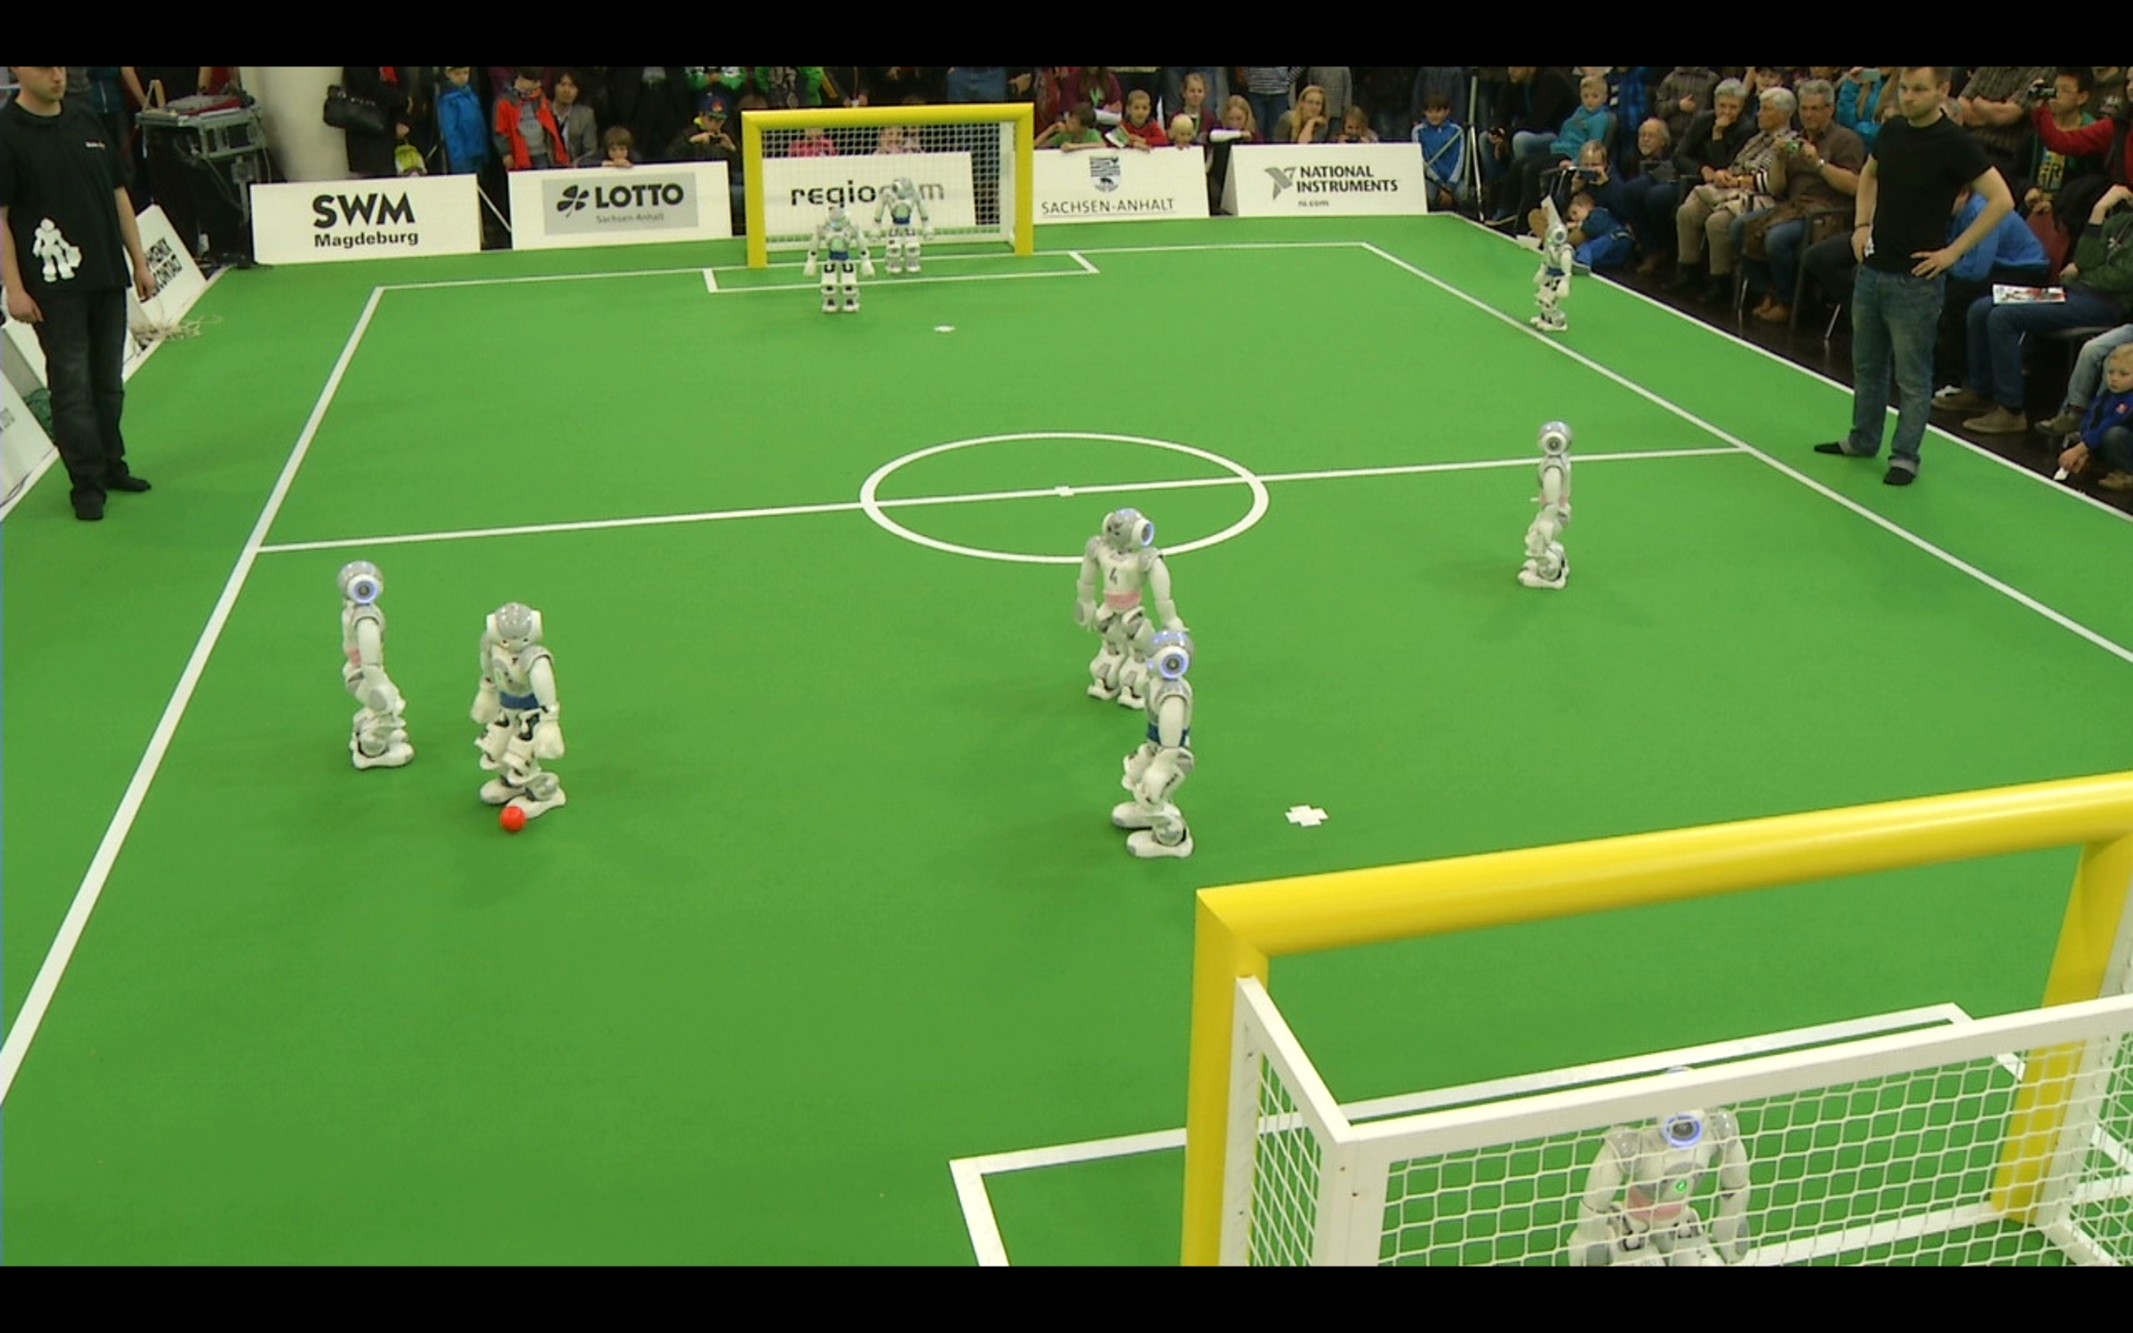
\includegraphics[scale=0.19]{Figures/Naos}
		};
	\end{tikzpicture}
	
\end{frame}

\begin{frame}
	\frametitle{Qualitative Evaluation on the Soccer Domain}
	\framesubtitle{RoboCup Iran Open}
	
	\begin{center}
		\href{run:../Scripts/nao.sh}
		{
			\begin{tikzpicture}
				\node at (0,0) [draw=black,ultra thick,inner sep=0pt]
				{
					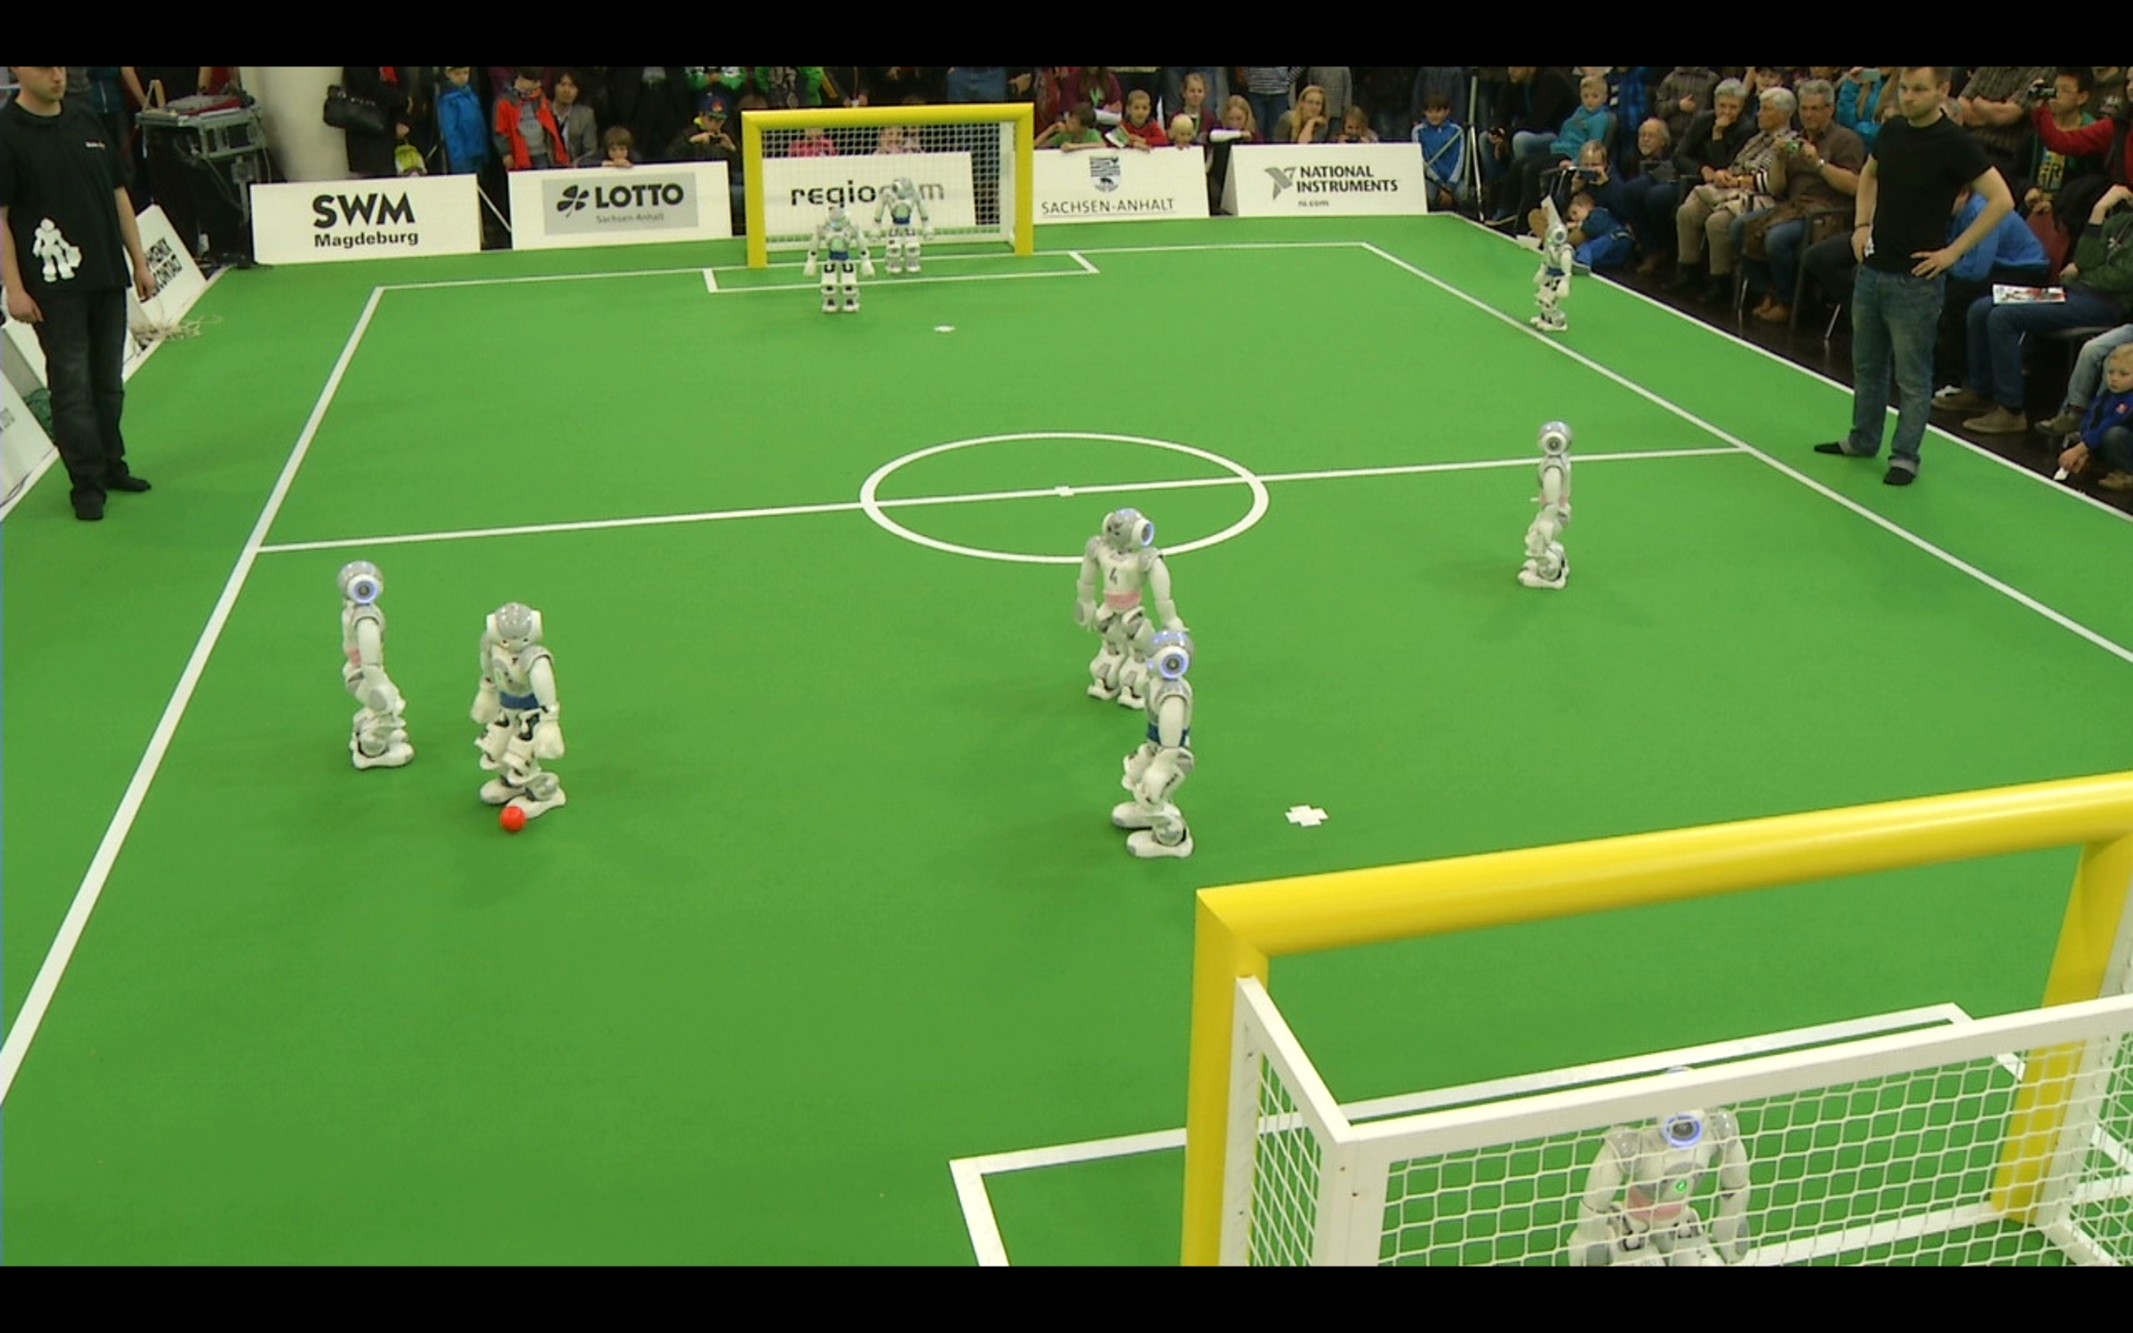
\includegraphics[width=0.65\linewidth]{Figures/Naos}
				};
			\end{tikzpicture}
		}
	\end{center}
\end{frame}

\begin{frame}
	\frametitle{Application Field}
	
	\vspace{-0.16cm}
	
	\begin{itemize}
		\item Multi-Agent, Multi-Object
	\end{itemize}
	
	\vspace{-0.45cm}
	
	\begin{columns}[t]
		\only<1->
		{
			\column{0.75\textwidth}
			
			\begin{block}{PETS 2009 data set}
				tracking of individuals within a crowd
			\end{block}
			
			\column{0.2\textwidth}
		}
	\end{columns}
	
	\centering
	\vspace{0.3cm}
	
	\begin{center}
		\begin{tikzpicture}
			\node at (0,0) [draw=black,ultra thick,inner sep=0pt]  {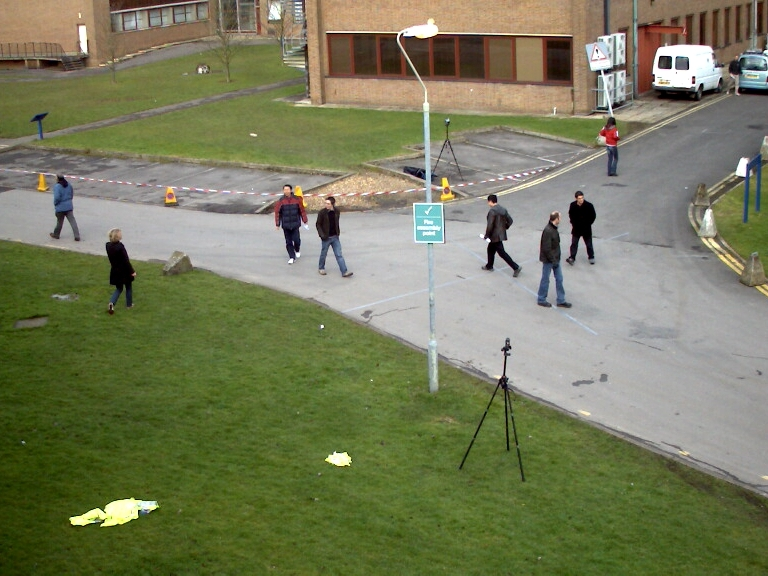
\includegraphics[height=2.85cm]{Figures/PETS2009-1}};
			\node at (4,0) [draw=black,ultra thick,inner sep=0pt]  {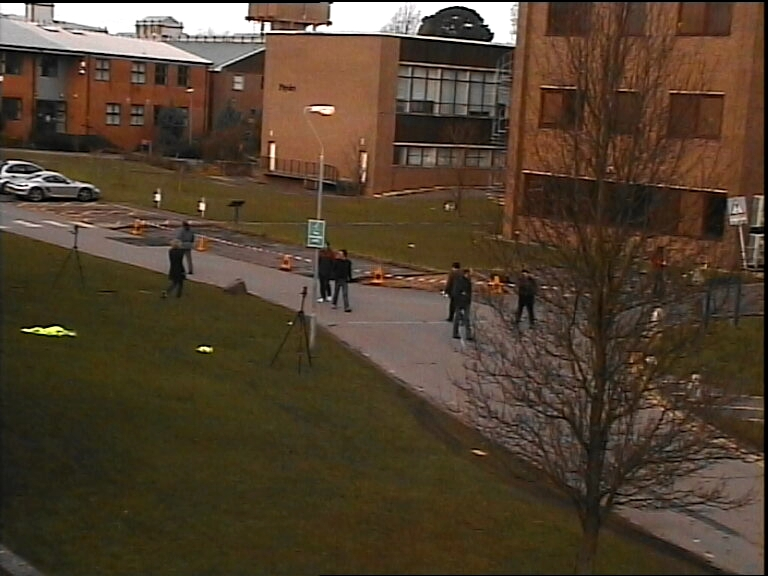
\includegraphics[height=2.85cm]{Figures/PETS2009-2}};
			\node at (8,0) [draw=black,ultra thick,inner sep=0pt]  {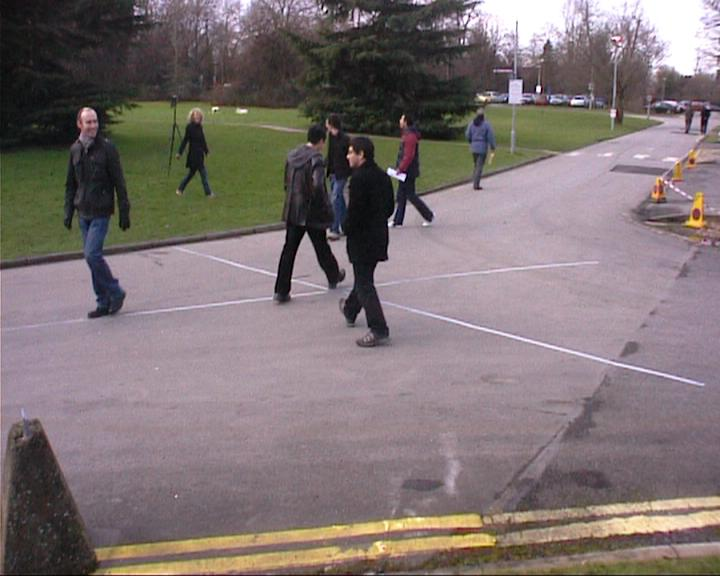
\includegraphics[height=2.85cm]{Figures/PETS2009-3}};
		\end{tikzpicture}
	\end{center}
\end{frame}

\begin{frame}
	\frametitle{Quantitative Evaluation on the People Domain}
	
	\begin{table}[!t]
		\renewcommand{\arraystretch}{1.3}
		\caption{Tracking performance on the PETS 2009 data set. MOTA (larger the better)
				 considers the number of missed detections, the number of false positives
				 and the switches of identities. MOTP (larger the better) considers the
				 precision of the detections.}
		\centering
		\vspace{0.2cm}
		
		\begin{tabular}{ccccc}
			\hline
			\hline
			\textbf{Method} & \textbf{MOTA} & \textbf{MOTP} & \textbf{Type} & \textbf{Real-Time} \\
			\hline
			Leal-Taix\'{e} \emph{et al.} & 0.67 & 0.594 & OFFLINE & NO \\
			\hline
			Berclaz \emph{et al.} & 0.732 & 0.651 & OFFLINE & NO \\
			\hline
			Sharma \emph{et al.} & 0.675 & 0.582 & OFFLINE & NO \\
			\hline
			Breitenstein \emph{et al.} & 0.745 & 0.563 & ONLINE & NO \\
			\hline
			Yang \emph{et al.} & 0.759 & 0.538 & ONLINE & NO \\
			\hline
			PTracking & \textbf{0.874} & \textbf{0.722} & ONLINE & \textbf{YES} \\
			\hline
		\hline
		\end{tabular}
	\end{table}
\end{frame}

\begin{frame}
	\frametitle{Application Field}
	
	\vspace{0.2cm}
	
	\begin{itemize}
		\item Multi-Agent, Multi-Object
	\end{itemize}
	
	\vspace{-0.45cm}
	
	\begin{columns}[t]
		\only<1->
		{
			\column{0.75\textwidth}
			
			\begin{block}{Inferring target goal}
				intention-inference for dynamic environments with multiple interactively navigating agents
			\end{block}
			
			\column{0.2\textwidth}
		}
	\end{columns}
	
	\centering
	
	\begin{center}
		\begin{tikzpicture}
			\node at (0,0) [draw=black,ultra thick,inner sep=0pt]  {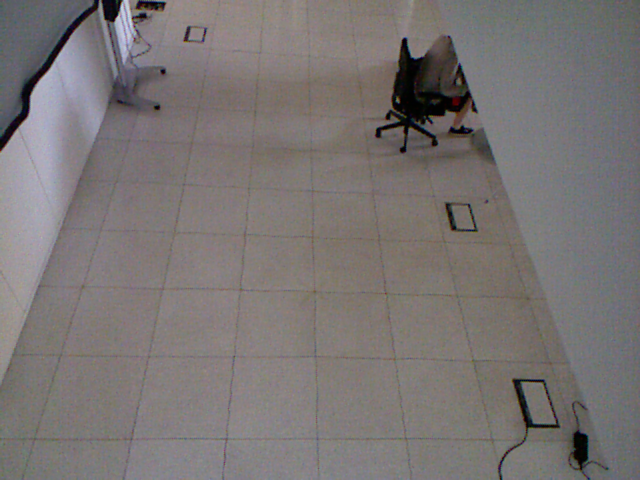
\includegraphics[height=2.9cm]{Figures/Kinect-1}};
			\node at (4,0) [draw=black,ultra thick,inner sep=0pt]  {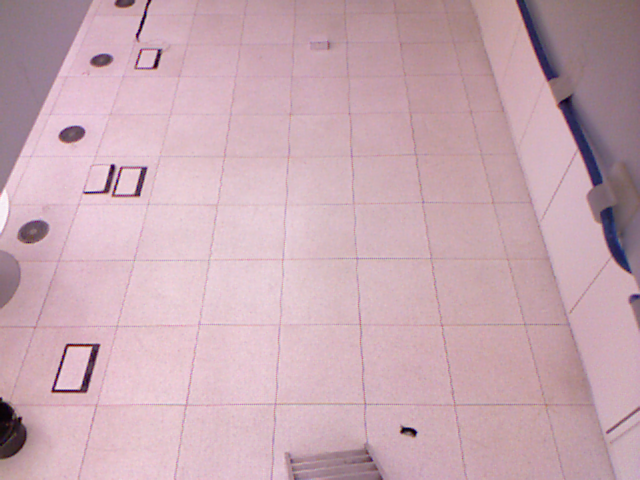
\includegraphics[height=2.9cm]{Figures/Kinect-2}};
			\node at (8,0) [draw=black,ultra thick,inner sep=0pt]  {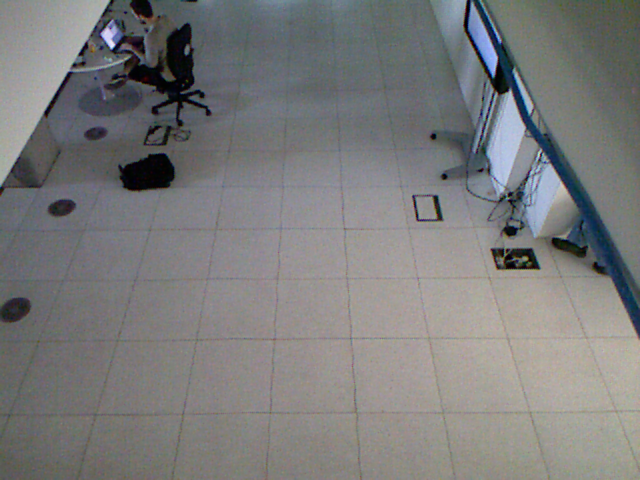
\includegraphics[height=2.9cm]{Figures/Kinect-3}};
		\end{tikzpicture}
	\end{center}
	
	\vspace{-0.3cm}
	
	\small
	This work has been realized during my visiting period at the University of Edinburgh, under the supervision of Prof. \emph{Subramanian Ramamoorthy}.
\end{frame}

\begin{frame}
	\frametitle{Qualitative Evaluation on the Inference Domain}
	\framesubtitle{InSpace - University of Edinburgh}
	
	\begin{center}
		\href{run:../Scripts/inspace.sh}
		{
			\begin{tikzpicture}
				\node at (0,0) [draw=black,ultra thick,inner sep=0pt]
				{
					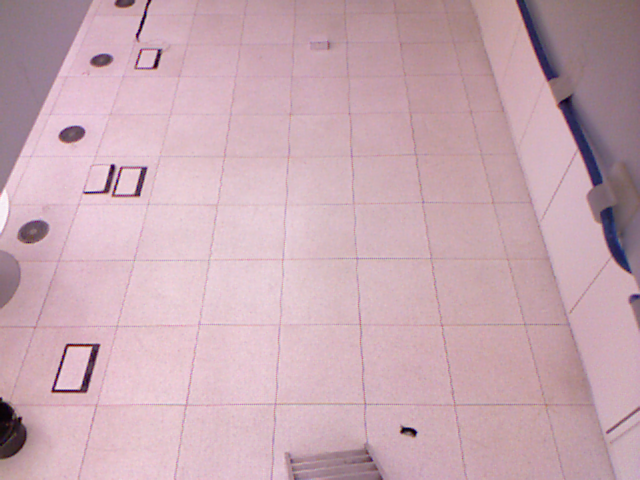
\includegraphics[width=0.65\linewidth]{Figures/Kinect-2.png}
				};
			\end{tikzpicture}
		}
	\end{center}
\end{frame}
